%%%%%%%%%%%%%%%%%%%%%%%%%%%%%%% beamer %%%%%%%%%%%%%%%%%%%%%%%%%%%%%%%%%%%%%%%%%%%%%%%%%
% To run - pdflatex filename.tex
%      acroread filename.pdf
%%%%%%%%%%%%%%%%%%%%%%%%%%%%%%%%%%%%%%%%%%%%%%%%%%%%%%%%%%%%%%%%%%%%%%%%%%%%%%%%%%%%%%%%

\documentclass[compress,oilve]{beamer}
\mode<presentation>

\usetheme[]{CambridgeUS}
% other themes: AnnArbor, Antibes, Bergen, Berkeley, Berlin, Boadilla, boxes, CambridgeUS, Copenhagen, Darmstadt, default, Dresden, Frankfurt, Goettingen,
% Hannover, Ilmenau, JuanLesPins, Luebeck, Madrid, Maloe, Marburg, Montpellier, PaloAlto, Pittsburg, Rochester, Singapore, Szeged, classic

\usecolortheme{beaver}
% color themes: albatross, beaver, beetle, crane, default, dolphin,  fly, lily, orchid, rose, seagull, seahorse, sidebartab, whale, wolverine

\usefonttheme{professionalfonts}
% font themes: default, professionalfonts, serif, structurebold, structureitalicserif, structuresmallcapsserif


\hypersetup{pdfpagemode=FullScreen} % makes your presentation go automatically to full screen

% define your own colors:
\definecolor{Red}{rgb}{1,0,0}
\definecolor{Blue}{rgb}{0,0,1}
\definecolor{Green}{rgb}{0,1,0}
\definecolor{magenta}{rgb}{1,0,.6}
\definecolor{lightblue}{rgb}{0,.5,1}
\definecolor{lightpurple}{rgb}{0.8, 0.6, 0.9}
\definecolor{gold}{rgb}{.6,.5,0}
\definecolor{orange}{rgb}{1,0.4,0}
\definecolor{hotpink}{rgb}{1,0,0.5}
\definecolor{newcolor2}{rgb}{.5,.3,.5}
\definecolor{newcolor}{rgb}{0,.3,1}
\definecolor{newcolor3}{rgb}{1,0,.35}
\definecolor{darkgreen1}{rgb}{0, .35, 0}
\definecolor{darkgreen}{rgb}{0, .6, 0}
\definecolor{darkred}{rgb}{.75,0,0}
\definecolor{skyblue}{HTML}{75bbfd}

\definecolor{olive}{cmyk}{0.64,0,0.95,0.4}
\definecolor{purpleish}{cmyk}{0.75,0.75,0,0}

% can also choose different themes for the "inside" and "outside"

% \usepackage{beamerinnertheme_______}
% inner themes include circles, default, inmargin, rectangles, rounded

% \usepackage{beamerouterthemesmoothbars}
% outer themes include default, infolines, miniframes, shadow, sidebar, smoothbars, smoothtree, split, tree


\useoutertheme[subsection=true, height=40pt]{smoothbars}

% to have the same footer on all slides
%\setbeamertemplate{footline}[text line]{STUFF HERE!}
\setbeamertemplate{footline}[text line]{} % makes the footer EMPTY
% include packages
%

%show the page numbers in footnote
%\addtobeamertemplate{navigation symbols}{}{%
%	\usebeamerfont{footline}%
%	\usebeamercolor[fg]{footline}%
%	\hspace{1em}%
%	\insertframenumber/\inserttotalframenumber
%}

\setbeamercolor{footline}{fg=purpleish}
\setbeamerfont{footline}{series=\bfseries}

%add color to curent subsection
\setbeamertemplate{section in head/foot}{\hfill\tikz\node[rectangle, fill=darkred, rounded corners=1pt,inner sep=1pt,] {\textcolor{white}{\insertsectionhead}};}
\setbeamertemplate{section in head/foot shaded}{\textcolor{darkred}{\hfill\insertsectionhead}}

% Remove bullet of subsections
\setbeamertemplate{headline}
{%
	\begin{beamercolorbox}{section in head/foot}
		\insertsectionnavigationhorizontal{\textwidth}{}{}
	\end{beamercolorbox}%
}


% modify headlline, specially headline size
\setbeamertemplate{headline}{%
	\leavevmode%
	\hbox{%
		\begin{beamercolorbox}[wd=\paperwidth,ht=3.5ex,dp=1.125ex]{palette quaternary}%
			\insertsectionnavigationhorizontal{\paperwidth}{}{\hskip0pt plus1filll}
		\end{beamercolorbox}%
	}
}

\setbeamertemplate{footline}{%
	\leavevmode%
	\hbox{\begin{beamercolorbox}[wd=.5\paperwidth,ht=2.5ex,dp=1.125ex,leftskip=.3cm plus1fill,rightskip=.3cm]{author in head/foot}%
			\usebeamerfont{author in head/foot}\insertshortauthor ~ \insertshortinstitute
		\end{beamercolorbox}%
		\begin{beamercolorbox}[wd=.5\paperwidth,ht=2.5ex,dp=1.125ex,leftskip=.3cm,rightskip=.3cm plus1fil]{title in head/foot}%
			\usebeamerfont{title in head/foot}\insertshorttitle\hfill\insertframenumber\,/\,\inserttotalframenumber
	\end{beamercolorbox}}%
	\vskip0pt%
}


%\setbeamertemplate{navigation symbols}{}

\title{CNN Architecture}
\author{ML Instruction Team, Fall 2022}
\institute[]{CE Department \newline  Sharif University of Technology \newline \newline \newline
            Ali Sharifi-Zarchi \newline
            Behrooz Azarkhalili \newline
            Arian Amani \newline
            Hamidreza Yaghobi}
\date[\today]{}
%\titlegraphic{\includegraphics[scale=.35]{example-image}}



%Write \usepackage{etex} just after the \documentclass line (it should be the first loaded package).
\usepackage{etex}
\usepackage{subcaption}
\usepackage{multicol}
\usepackage{amsmath}
\usepackage{epsfig}
\usepackage{graphicx}
\usepackage[all,knot]{xy}
\xyoption{arc}
\usepackage{url}
\usepackage{multimedia}
\usepackage{hyperref}
\hypersetup{colorlinks,linkcolor=blue,citecolor=redorange,urlcolor=darkred}
\usepackage{multirow}
\usepackage[font={scriptsize}]{caption}
\usepackage{pgf}
\usepackage{fontspec}
\usepackage[clean]{svg}
\usepackage{xcolor}


%\setsansfont[Scale=MatchLowercase, BoldFont = * Bold, ItalicFont = * Italic]{Caladea}

%\usepackage{enumitem,xcolor}
%\newcommand{\labelitemi}{$\blacksquare$}
%\newcommand{\labelitemii}{$\diamond$}
%\newcommand{\labelitemiii}{$\square$}
%\newcommand{\labelitemiv}{$\ast$}
%\setbeamercolor*{item}{fg=red}


\usefonttheme{professionalfonts} 
\setbeamertemplate{itemize item}{\color{skyblue}$\blacksquare$}
\setbeamertemplate{itemize subitem}{\color{hotpink}$\blacktriangleright$}
\setbeamertemplate{itemize subsubitem}{\color{orange}$\bullet$}


\usepackage{anyfontsize}
\usepackage{t1enc}
\usepackage{tikz}
\usetikzlibrary{calc,trees,positioning,arrows,chains,shapes.geometric,decorations.pathreplacing,decorations.pathmorphing,shapes,matrix,shapes.symbols}



\newtheorem{proposition}[theorem]{Proposition}
\newtheorem{remark}[theorem]{Remark}
\newtheorem{assumption}[theorem]{Assumption}

\usepackage{fontspec,unicode-math}
\setmainfont{Consolas}[
    Scale=0.9,
    Path=./Fonts/,
    Extension = .ttf,
]
\setmonofont{Monaco}[
    Scale=0.9,
    Path=./Fonts/,
    Extension = .ttf,
]

\setsansfont[Scale=1]{Times New Roman}

%\usepackage{smartdiagram}
%\usesmartdiagramlibrary{additions}
%%%%%%%%%%%%%%%%%%%%%%%%%%%%%%%%%%%%%%%%%%%%%%%%%%%%%%%%%%%%%%%%%%%%%%%%%%%%%%%%%%%%%%%%%%%%
%%%%%%%%%%%%%%%%%%%%%%%%%%%%%% Title Page Info %%%%%%%%%%%%%%%%%%%%%%%%%%%%%%%%%%%%%%%%%%%
%%%%%%%%%%%%%%%%%%%%%%%%%%%%%%%%%%%%%%%%%%%%%%%%%%%%%%%%%%%%%%%%%%%%%%%%%%%%%%%%%%%%%%%%%%


%%%%%%%%%%%%%%%%%%%%%%%%%%%%%%%%%%%%%%%%%%%%%%%%%%%%%%%%%%%%%%%%%%%%%%%%%%%%%%%%%%%%%%%%%%
%%%%%%%%%%%%%%%%%%%%%%%%%%%%%% Begin Your Document %%%%%%%%%%%%%%%%%%%%%%%%%%%%%%%%%%%%%%%
%%%%%%%%%%%%%%%%%%%%%%%%%%%%%%%%%%%%%%%%%%%%%%%%%%%%%%%%%%%%%%%%%%%%%%%%%%%%%%%%%%%%%%%%%%
\begin{document}
	
%%%%%%%%%%%%%%%%%%%%%%%%%%%%%%%%%%%%%%%%%%%%%%%%%%%%%%%%%%%%%%%%%%%%%%%%%%%%%%%%%%%%%%%%%%
	\fontsize{9}{9}
\begin{frame}[noframenumbering, plain]
	\titlepage
\end{frame}

%%%%%%%%%%%%%%%%%%%%%%%%%%%%%%%%%%%%%%%%%%%%%%%%%%%%%%%%%%%%%%%%%%%%%%%%%%%%%%%%%%%%%%%%%%
\section{Introduction}
%%%%%%%%%%%%%%%%%%%%%%%%%%%%%%%%%%%%%%%%%%%%%%%%%%%%%%%%%%%%%%%%%%%%%%%%######
\frame{\frametitle{Convolutional Neural Networks: History}
\Large{Biological Inspiration of Convolutional Neural Networks}
\newline \newline
\large{\textbf{Hubel and Wiesel}}

\begin{itemize}
	\item 1959
	\item 1961
	\item 1968

\end{itemize}	
	
}

%%%%%%%%%%%%%%%%%%%%%%%%%%%%%%%%%%%%%%%%%%%%%%%%%%%%%%%%%%%%%%%%%%%%%%%%%%%%%%%%%%%%%%%%%%%%%%%
\section{Kernels}
%%%%%%%%%%%%%%%%%%%%%%%%%%%%%%%%%%%%%%%%%%%%%%%%%%%%%%%%%%%%%%%%%%%%%%%%%%%%%%%%%%%%%%%%%%%%%%%

\frame{\frametitle{CNNs}

\Large{What we've been using:}
\newline
\large{Fully Connected Layers}
\newline
\begin{figure}
    \centering
    \includesvg[width=1\columnwidth]{images/nn.svg}
\end{figure}



}

%%%%%%%%%%%%%%%%%%%%%%%%%%%%%%%%%%%%%%%%%%%%%%%%%%%%%%%%%%%%%%%%%%%%%%%%%%%%%%%%%%%%%%%%%%%%%%%

\frame{\frametitle{CNNs}

\Large{What we're going to learn:}
\newline
\large{Convolutional Layer}
\newline
\begin{figure}
    \centering
    \includesvg[width=0.6\columnwidth]{images/CNN1.svg}
\end{figure}

}
%%%%%%%%%%%%%%%%%%%%%%%%%%%%%%%%%%%%%%%%%%%%%%%%%%%%%%%%%%%%%%%%%%%%%%%%%%%%%%%%%%%%%%%%%%%%%%%

\frame{\frametitle{CNNs}

\large{Convolutional Layer}
\newline

\begin{itemize}
	\item Filters always extend the full depth of the input volume.\newline
	(\#Input channels == \#Filter Channels)
\end{itemize}	

\begin{figure}
    \centering
    \includesvg[width=0.6\columnwidth]{images/CNN2.svg}
\end{figure}

}

%%%%%%%%%%%%%%%%%%%%%%%%%%%%%%%%%%%%%%%%%%%%%%%%%%%%%%%%%%%%%%%%%%%%%%%%%%%%%%%%%%%%%%%%%%%%%%%
\section{Strides}
%%%%%%%%%%%%%%%%%%%%%%%%%%%%%%%%%%%%%%%%%%%%%%%%%%%%%%%%%%%%%%%%%%%%%%%%%%%%%%%%%%%%%%%%%%%%%%%

\frame{\frametitle{What is a Stride}

\Large{The amount of movement between applications of the filter to the input image is referred to as the stride, and it is almost always symmetrical in height and width dimensions.}
\newline
\newline
\normalsize{Closer look}
\begin{itemize}
	\item 7x7 input with 3x3 filter
\end{itemize}	

\begin{figure}
    \centering
    \includesvg[width=0.35\columnwidth]{images/Stride1.svg}
\end{figure}

}

%%%%%%%%%%%%%%%%%%%%%%%%%%%%%%%%%%%%%%%%%%%%%%%%%%%%%%%%%%%%%%%%%%%%%%%%%%%%%%%%%%%%%%%%%%%%%%%

\frame{\frametitle{What is a Stride}

\Large{The amount of movement between applications of the filter to the input image is referred to as the stride, and it is almost always symmetrical in height and width dimensions.}
\newline
\newline
\normalsize{Closer look}
\begin{itemize}
	\item 7x7 input with 3x3 filter
\end{itemize}	

\begin{figure}
    \centering
    \includesvg[width=0.35\columnwidth]{images/Stride2.svg}
\end{figure}

}

%%%%%%%%%%%%%%%%%%%%%%%%%%%%%%%%%%%%%%%%%%%%%%%%%%%%%%%%%%%%%%%%%%%%%%%%%%%%%%%%%%%%%%%%%%%%%%%

\frame{\frametitle{What is a Stride}

\Large{The amount of movement between applications of the filter to the input image is referred to as the stride, and it is almost always symmetrical in height and width dimensions.}
\newline
\newline
\normalsize{Closer look}
\begin{itemize}
	\item 7x7 input with 3x3 filter
\end{itemize}	

\begin{figure}
    \centering
    \includesvg[width=0.35\columnwidth]{images/Stride3.svg}
\end{figure}

}

%%%%%%%%%%%%%%%%%%%%%%%%%%%%%%%%%%%%%%%%%%%%%%%%%%%%%%%%%%%%%%%%%%%%%%%%%%%%%%%%%%%%%%%%%%%%%%%

\frame{\frametitle{What is a Stride}

\Large{The amount of movement between applications of the filter to the input image is referred to as the stride, and it is almost always symmetrical in height and width dimensions.}
\newline
\newline
\normalsize{Closer look}
\begin{itemize}
	\item 7x7 input with 3x3 filter
\end{itemize}	

\begin{figure}
    \centering
    \includesvg[width=0.35\columnwidth]{images/Stride4.svg}
\end{figure}

}

%%%%%%%%%%%%%%%%%%%%%%%%%%%%%%%%%%%%%%%%%%%%%%%%%%%%%%%%%%%%%%%%%%%%%%%%%%%%%%%%%%%%%%%%%%%%%%%

\frame{\frametitle{What is a Stride}

\Large{The amount of movement between applications of the filter to the input image is referred to as the stride, and it is almost always symmetrical in height and width dimensions.}
\newline
\newline
\normalsize{Closer look}
\begin{itemize}
	\item 7x7 input with 3x3 filter
	\item This was a Stride 1 filter
	\item=> Outputs 5x5
\end{itemize}	

\begin{figure}
    \centering
    \includesvg[width=0.3\columnwidth]{images/Stride5.svg}
\end{figure}

}


%%%%%%%%%%%%%%%%%%%%%%%%%%%%%%%%%%%%%%%%%%%%%%%%%%%%%%%%%%%%%%%%%%%%%%%%%%%%%%%%%%%%%%%%%%%%%%%

\frame{\frametitle{Stride}

\newline
\newline
\normalsize{\color{red}Now let's use Stride 2}
\begin{itemize}
	\item 7x7 input with 3x3 filter

\end{itemize}	

\begin{figure}
    \centering
    \includesvg[width=0.35\columnwidth]{images/Stride6.svg}
\end{figure}

}

%%%%%%%%%%%%%%%%%%%%%%%%%%%%%%%%%%%%%%%%%%%%%%%%%%%%%%%%%%%%%%%%%%%%%%%%%%%%%%%%%%%%%%%%%%%%%%%

\frame{\frametitle{Stride}

\newline
\newline
\normalsize{Now let's use Stride 2}
\begin{itemize}
	\item 7x7 input with 3x3 filter

\end{itemize}	

\begin{figure}
    \centering
    \includesvg[width=0.35\columnwidth]{images/Stride7.svg}
\end{figure}
}

%%%%%%%%%%%%%%%%%%%%%%%%%%%%%%%%%%%%%%%%%%%%%%%%%%%%%%%%%%%%%%%%%%%%%%%%%%%%%%%%%%%%%%%%%%%%%%%

\frame{\frametitle{Stride}

\newline
\newline
\normalsize{Now let's use Stride 2}
\begin{itemize}
	\item 7x7 input with 3x3 filter
	\item This was a Stride 2 filter
	\item=> Outputs 3x3
\end{itemize}	

\begin{figure}
    \centering
    \includesvg[width=0.3\columnwidth]{images/Stride8.svg}
\end{figure}
}

%%%%%%%%%%%%%%%%%%%%%%%%%%%%%%%%%%%%%%%%%%%%%%%%%%%%%%%%%%%%%%%%%%%%%%%%%%%%%%%%%%%%%%%%%%%%%%%

\frame{\frametitle{Stride}

\newline
\newline
\normalsize{\color{red}Stride 3?}
\begin{itemize}
	\item 7x7 input with 3x3 filter

\end{itemize}	

\begin{figure}
    \centering
    \includesvg[width=0.25\columnwidth]{images/Stride9.svg}
    \includesvg[width=0.25\columnwidth]{images/Stride10.svg}
    \includesvg[width=0.34\columnwidth]{images/Stride11.svg}
\end{figure}
}
%%%%%%%%%%%%%%%%%%%%%%%%%%%%%%%%%%%%%%%%%%%%%%%%%%%%%%%%%%%%%%%%%%%%%%%%%%%%%%%%%%%%%%%%%%%%%%%

\frame{\frametitle{Stride}

\newline
\newline
\normalsize{\color{red}So 7x7 input with 3x3 filter and stride 3 doens't work!}
\newline
\newline
\large{Let't do the calculations:}
\newline \newline
\large{$Output Size = (N - F) / Stride + 1$}

\begin{figure}
    \centering
    \includesvg[width=0.4\columnwidth]{images/Stride12.svg}
\end{figure}
}

%%%%%%%%%%%%%%%%%%%%%%%%%%%%%%%%%%%%%%%%%%%%%%%%%%%%%%%%%%%%%%%%%%%%%%%%%%%%%%%%%%%%%%%%%%%%%%%

\frame{\frametitle{Stride}

\newline
\newline
\large{$Output Size = (N - F) / Stride + 1$}

N = 7, F = 3 =>
\begin{itemize}
    \item Stride 1 ==> $(7 - 3) / 1 + 1 = 5$
    \item Stride 2 ==> $(7 - 3) / 2 + 1 = 3$
    \item \color{red}Stride 3 ==> $(7 - 3) / 3 + 1 = 2.33$ :))
\end{itemize}
\begin{figure}
    \centering
    \includesvg[width=0.4\columnwidth]{images/Stride12.svg}
\end{figure}
}

%%%%%%%%%%%%%%%%%%%%%%%%%%%%%%%%%%%%%%%%%%%%%%%%%%%%%%%%%%%%%%%%%%%%%%%%%%%%%%%%%%%%%%%%%%%%%%%
\frame{\frametitle{Strides}
\begin{center}
    \LARGE{Do you see any problems?}
\end{center}
}

%%%%%%%%%%%%%%%%%%%%%%%%%%%%%%%%%%%%%%%%%%%%%%%%%%%%%%%%%%%%%%%%%%%%%%%%%%%%%%%%%%%%%%%%%%%%%%%
\frame{\frametitle{Strides}
\begin{center}
    \begin{itemize}
        \item\color{red}\Large{1. Borders don't get enough attention.}
    \end{itemize}
    \begin{figure}
        \centering
        \includesvg[width=0.9\columnwidth]{images/padding1.svg}
        \caption{\hyperlink{https://d2l.ai/chapter_convolutional-neural-networks/padding-and-strides.html#img-conv-reuse}{Dive into Deep Learning, Fig. 7.3.1: }Pixel utilization for convolutions of size $1 \times 1$, $2 \times 2$, and $3 \times 3$ respectively.}
        % \label{fig:my_label}
    \end{figure}
\end{center}
}

%%%%%%%%%%%%%%%%%%%%%%%%%%%%%%%%%%%%%%%%%%%%%%%%%%%%%%%%%%%%%%%%%%%%%%%%%%%%%%%%%%%%%%%%%%%%%%%
\frame{\frametitle{Strides}
\begin{center}
    \begin{itemize}
        \item\Large{1. Borders don't get enough attention.}
        \item\color{red}\Large{2. Outputs shrink!}
    \end{itemize}
    \begin{figure}
        \centering
        \includesvg[width=0.9\columnwidth]{images/Padding2.svg}
        \caption{32x32 input shrinks to 28x28 output. (information loss)}
        % \label{fig:my_label}
    \end{figure}
\end{center}
}

%%%%%%%%%%%%%%%%%%%%%%%%%%%%%%%%%%%%%%%%%%%%%%%%%%%%%%%%%%%%%%%%%%%%%%%%%%%%%%%%%%%%%%%%%%%%%%%
\frame{\frametitle{Strides}
\begin{center}
    \LARGE{What is the solution?}
\end{center}
}
%%%%%%%%%%%%%%%%%%%%%%%%%%%%%%%%%%%%%%%%%%%%%%%%%%%%%%%%%%%%%%%%%%%%%%%%%%%%%%%%%%%%%%%%%%%%%%%
\section{Padding}
%%%%%%%%%%%%%%%%%%%%%%%%%%%%%%%%%%%%%%%%%%%%%%%%%%%%%%%%%%%%%%%%%%%%%%%%%%%%%%%%%%%%%%%%%%%%%%%
\frame{\frametitle{Padding}
\begin{center}
    \LARGE{Enters Padding}
\end{center}
}

%%%%%%%%%%%%%%%%%%%%%%%%%%%%%%%%%%%%%%%%%%%%%%%%%%%%%%%%%%%%%%%%%%%%%%%%%%%%%%%%%%%%%%%%%%%%%%%
\frame{\frametitle{Padding}
\begin{center}
    \begin{itemize}
        \item\large{We can use Padding to preserve the dimensionality}
        \item\large{It ensures that all pixels are used equally frequently}
    \end{itemize}
    \begin{figure}
        \centering
        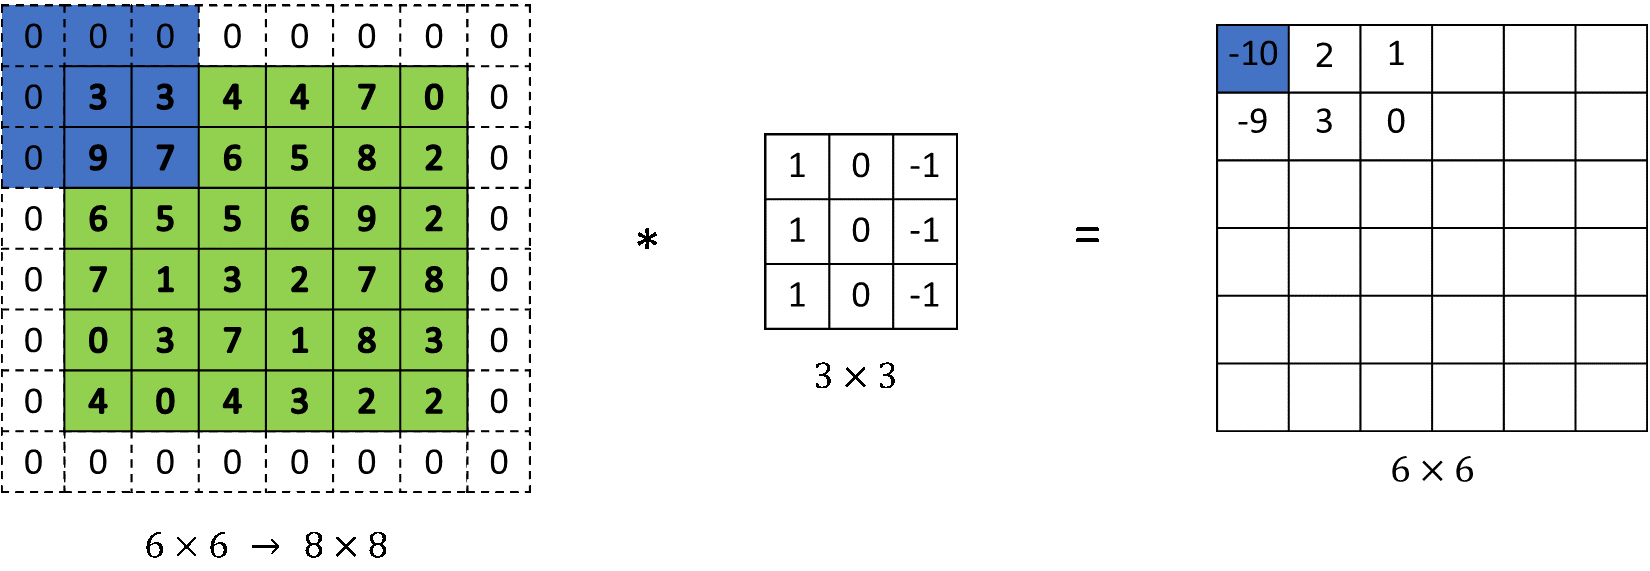
\includegraphics[width=0.9\columnwidth]{images/Padding3.png}
        \caption{\hyperlink{https://datahacker.rs/what-is-padding-cnn/}{DataHacker.rs: CNN Padding - }Applying padding of 1 before convolving with $3 \times 3$ filter}
        % \label{fig:my_label}
    \end{figure}
\end{center}
}

%%%%%%%%%%%%%%%%%%%%%%%%%%%%%%%%%%%%%%%%%%%%%%%%%%%%%%%%%%%%%%%%%%%%%%%%%%%%%%%%%%%%%%%%%%%%%%%
\frame{\frametitle{Padding}
\begin{center}
    \begin{itemize}
        \item\color{red}\large{It is common to use $P = (F - 1) / 2$ with stride 1 to preserve the input size.}
    \end{itemize}
    \begin{figure}
        \centering
        \includesvg[width=0.4\columnwidth]{images/Padding4.svg}
        \caption{Applying zero-padding to a 7x7 input with padding 1}
        % \label{fig:my_label}
    \end{figure}
\end{center}
}

%%%%%%%%%%%%%%%%%%%%%%%%%%%%%%%%%%%%%%%%%%%%%%%%%%%%%%%%%%%%%%%%%%%%%%%%%%%%%%%%%%%%%%%%%%%%%%%
\frame{\frametitle{Padding}
\begin{center}
    \begin{itemize}
        \item\large{It is common to use $P = (F - 1) / 2$ with stride 1 to preserve the input size.}
        \item\color{red}\large{$OutputSize = (N + 2P - F) / Stride + 1$}
        \end{itemize}
    \begin{figure}
        \centering
        \includesvg[width=0.4\columnwidth]{images/Padding4.svg}
        \caption{Applying zero-padding to a 7x7 input with padding 1}
        % \label{fig:my_label}
    \end{figure}
\end{center}
}

%%%%%%%%%%%%%%%%%%%%%%%%%%%%%%%%%%%%%%%%%%%%%%%%%%%%%%%%%%%%%%%%%%%%%%%%%%%%%%%%%%%%%%%%%%%%%%%
\frame{\frametitle{Padding}
\begin{center}
    \begin{itemize}
        \item\large{It is common to use $P = (F - 1) / 2$ with stride 1 to preserve the input size.}
        \item\large{$OutputSize = (N + 2P - F) / Stride + 1$}
        \newline
    \end{itemize}
    \begin{minipage}{0.5\textwidth}
        \begin{figure}
            \centering
            \includesvg[width=0.7\columnwidth]{images/Padding4.svg}
            \caption{Applying zero-padding to a 7x7 input with padding 1}
        \end{figure}

    \end{minipage} \hfill
    \begin{minipage}{0.45\textwidth}
        \large{\color{red}7x7 input, stride 1, P to preserve the dimentions?}
        \begin{itemize}
            \item $F = 3 --> P = 1$
            \item $F = 5 --> P = 2$
            \item $F = 7 --> P = 3$
        \end{itemize}
    \end{minipage}
    
\end{center}
}

%%%%%%%%%%%%%%%%%%%%%%%%%%%%%%%%%%%%%%%%%%%%%%%%%%%%%%%%%%%%%%%%%%%%%%%%%%%%%%%%%%%%%%%%%%%%%%%
\section{Channels, etc.}
%%%%%%%%%%%%%%%%%%%%%%%%%%%%%%%%%%%%%%%%%%%%%%%%%%%%%%%%%%%%%%%%%%%%%%%%%%%%%%%%%%%%%%%%%%%%%%%
\frame{\frametitle{Channels, etc.}
\begin{center}
    \LARGE{HI :))}
\end{center}
}
%%%%%%%%%%%%%%%%%%%%%%%%%%%%%%%%%%%%%%%%%%%%%%%%%%%%%%%%%%%%%%%%%%%%%%%%%%%%%%%%%%%%%%%%%%%%%%%
\frame{\frametitle{Final Notes}
\centering
\vspace{50 pt}
\textbf{Thank You!}
\vspace{50pt}

\textbf{Any Question?}
}
%%%%%%%%%%%%%%%%%%%%%%%%%%%%%%%%%%%%%%%%%%
\end{document}